% =============================================================================
% Module 8: Non-Axisymmetric Models and Critical Curves
% =============================================================================
% Sources: Congdon & Keeton Ch. 4.5 & 6.1, Narayan & Bartelmann Sec. 3.5,
%          Saha et al., Petters, Levine & Wambsganss (2001)
% Mathematica: ../Mathematica/08_Elliptical_Models_Caustics/
% =============================================================================

\chapter{Non-Axisymmetric Models and Critical Curves}
\label{ch:elliptical_models}

\begin{quote}
\textit{Breaking circular symmetry in the lens model produces the rich
phenomenology of strong lensing: quadruply imaged quasars, Einstein
crosses, giant luminous arcs.  The structure of critical curves and
caustics determines everything --- how many images form, where they
appear, how bright they are, and even which direction they face.}
\hfill --- adapted from Congdon \& Keeton (2018)
\end{quote}

\noindent
In Modules~\ref{ch:magnification} and~\ref{ch:axisymmetric_models} we
developed the Jacobian formalism for magnification and applied it to
axisymmetric lens models: the point mass and the singular isothermal
sphere (SIS).  These models have a continuous rotational symmetry that
makes the mathematics tractable but the phenomenology limited.  The SIS,
for instance, can produce at most two images of a point source, and its
critical curve is a perfect circle.

Real galaxies, however, are \textit{elliptical}.  Their mass
distributions have axis ratios $q \sim 0.5$--$0.9$, and they live in
environments that contribute external tidal shear.  Breaking circular
symmetry introduces qualitatively new phenomena:
\begin{itemize}[nosep]
    \item Critical curves deform from circles into ellipses and ovals.
    \item Caustics develop a \textbf{diamond (astroid)} shape with
          cusps and folds.
    \item Sources can be \textbf{quadruply imaged} (not just doubly),
          producing Einstein crosses and arcs.
    \item The \textbf{topology} of image configurations --- how many
          images exist, their parities, and their magnifications ---
          is entirely governed by the source's position relative to
          the caustic structure.
\end{itemize}

This module introduces the two workhorse non-axisymmetric models
(SIS + external shear and the singular isothermal ellipsoid) and then
develops the theory of critical curves, caustics, and image topology
in full detail.  The image topology section is the conceptual heart
of strong lensing theory.

\medskip
\noindent
\textbf{Companion Mathematica files:}
\begin{itemize}[nosep]
    \item \mathlink{08_Elliptical_Models_Caustics/critical\_curves\_caustics.wl}{critical\_curves\_caustics.wl}
          --- symbolic and numerical computation of critical curves
          and caustics for SIS+shear and SIE models; image position
          solver; figure generation for all module figures
    \item \mathlink{08_Elliptical_Models_Caustics/image\_configurations.nb}{image\_configurations.nb}
          --- interactive notebook: place a source on the source
          plane and watch images appear, colored by parity; animate
          caustic crossings; sliders for ellipticity and shear
\end{itemize}


% =====================================================================
\section{Introduction: Why Non-Axisymmetric Models Matter}
\label{sec:elliptical_intro}

The singular isothermal sphere (Module~\ref{ch:axisymmetric_models}) is
an excellent starting point for galaxy-scale lensing.  Its velocity
dispersion $\sigma_v$ maps directly onto observable galaxy kinematics,
and its Einstein radius $\thetaE = 4\pi\sigma_v^2 \Dds/(\speedoflight^2
\Ds)$ sets the angular scale of lensing.  But the SIS has a fundamental
limitation: perfect circular symmetry.

Observations of strong lens systems reveal:
\begin{enumerate}
    \item \textbf{Quadruple images} are common.  About 20--30\% of
          known galaxy-scale lens systems are quads (four bright images
          plus a faint central image), which an SIS cannot produce.
    \item \textbf{Giant luminous arcs} in galaxy clusters are
          tangentially stretched images that trace out the critical
          curves of the cluster potential.  These arcs are not perfect
          circles, implying the mass distribution is not axisymmetric.
    \item \textbf{Astrometric anomalies} in lens models require
          ellipticity and/or external shear to achieve acceptable fits.
\end{enumerate}

The simplest way to break axial symmetry is to add a constant
\textbf{external shear} to the SIS potential.  The resulting
SIS + shear model already captures the essential features: diamond
caustics, quad images, and fold/cusp configurations.  The more
physically motivated \textbf{singular isothermal ellipsoid} (SIE)
achieves the same through an intrinsically elliptical mass
distribution and is the model used in modern lens-modeling codes
such as \texttt{lenstronomy} and \texttt{PyAutoLens}.


% =====================================================================
\section{SIS + External Shear}
\label{sec:sis_shear}

The simplest non-axisymmetric lens model augments the SIS potential
with a constant external tidal shear $\gamma_{\mathrm{ext}}$.
Physically, this shear arises from the tidal gravitational field of
neighboring galaxies or the cluster environment in which the lens
galaxy resides.

\subsection{Lensing Potential}

The lensing potential is
(Congdon \& Keeton eq.~6.7):
\begin{equation}
    \boxed{
    \psiL(\vectheta) = \thetaE\,|\vectheta|
    + \frac{1}{2}\,\gamma_{\mathrm{ext}}\,
    (\theta_1^2 - \theta_2^2)
    }
    \label{eq:psi_sis_shear}
\end{equation}
where $|\vectheta| = \sqrt{\theta_1^2 + \theta_2^2}$ and we have
chosen the shear to be aligned with the $\theta_1$-axis (the general
case involves a rotation by the shear angle $\phi_\gamma$).  The
first term is the SIS potential; the second is the external shear
contribution.

\subsection{Deflection Angle}

The deflection angle components are:
\begin{equation}
    \alpha_1 = \frac{\partial\psiL}{\partial\theta_1}
    = \thetaE\,\frac{\theta_1}{|\vectheta|}
    + \gamma_{\mathrm{ext}}\,\theta_1 \,,
    \qquad
    \alpha_2 = \frac{\partial\psiL}{\partial\theta_2}
    = \thetaE\,\frac{\theta_2}{|\vectheta|}
    - \gamma_{\mathrm{ext}}\,\theta_2 \,.
    \label{eq:alpha_sis_shear}
\end{equation}
The SIS contribution deflects radially inward; the shear contribution
stretches along $\theta_1$ and compresses along $\theta_2$ (for
$\gamma_{\mathrm{ext}} > 0$).

\subsection{Convergence and Shear}

The convergence of the SIS + shear model is the same as the pure SIS
(the external shear does not add mass):
\begin{equation}
    \kappab(\vectheta) = \frac{\thetaE}{2\,|\vectheta|} \,.
    \label{eq:kappa_sis_shear}
\end{equation}
The total shear now has contributions from both the SIS and the
external shear.  For the SIS alone,
$|\gammaL_{\mathrm{SIS}}| = \thetaE/(2|\vectheta|) = \kappab$.
The external shear adds $\gamma_{\mathrm{ext}}$ aligned with the
coordinate axes, so the total shear field is anisotropic and
position-dependent.

\subsection{Critical Curves}

The critical curves are defined by $\det\Amat = 0$.  For the
SIS + shear model, the condition becomes (working in polar
coordinates $\theta_1 = \theta\cos\phi$,
$\theta_2 = \theta\sin\phi$):
\begin{equation}
    \boxed{
    \theta_{\mathrm{crit}}(\phi)
    = \frac{\thetaE}{1 - \gamma_{\mathrm{ext}}^2
    - 2\,\gamma_{\mathrm{ext}}\cos 2\phi}
    \cdot (1 - \gamma_{\mathrm{ext}}\cos 2\phi)
    }
    \label{eq:crit_sis_shear}
\end{equation}
For $\gamma_{\mathrm{ext}} = 0$ this reduces to $\theta = \thetaE$
(the SIS critical circle).  For $\gamma_{\mathrm{ext}} > 0$, the
critical curve is an \textbf{ellipse}: elongated along the
$\theta_2$-axis (perpendicular to the shear direction) and compressed
along $\theta_1$.

\begin{remark}
The critical curve is elongated \textit{perpendicular} to the shear
direction.  This is physically intuitive: the shear stretches images
along $\theta_1$, which means the magnification diverges at smaller
$\theta$ in that direction, pushing the critical curve inward along
$\theta_1$ and outward along $\theta_2$.
\end{remark}

\subsection{Caustics: The Diamond (Astroid)}

The caustics are obtained by mapping the critical curves through the
lens equation $\vecbeta = \vectheta_{\mathrm{crit}} -
\vecalpha(\vectheta_{\mathrm{crit}})$.  For the SIS + shear model,
the tangential caustic takes the shape of a \textbf{diamond} or
\textbf{astroid} --- a four-cusped curve.

In parametric form, the caustic is:
\begin{align}
    \beta_1(\phi) &= \theta_{\mathrm{crit}}(\phi)\cos\phi
    - \thetaE\cos\phi - \gamma_{\mathrm{ext}}\,
    \theta_{\mathrm{crit}}(\phi)\cos\phi \,,
    \label{eq:caustic_sis_shear_1} \\
    \beta_2(\phi) &= \theta_{\mathrm{crit}}(\phi)\sin\phi
    - \thetaE\sin\phi + \gamma_{\mathrm{ext}}\,
    \theta_{\mathrm{crit}}(\phi)\sin\phi \,.
    \label{eq:caustic_sis_shear_2}
\end{align}
This curve has four cusps (at $\phi = 0, \pi/2, \pi, 3\pi/2$) and
four fold segments connecting them.  The size of the diamond is
proportional to $\gamma_{\mathrm{ext}}$: for
$\gamma_{\mathrm{ext}} = 0$, the caustic degenerates to a point
(the SIS point caustic), and for larger shear values, the diamond
grows.

\begin{figure}[ht]
    \centering
    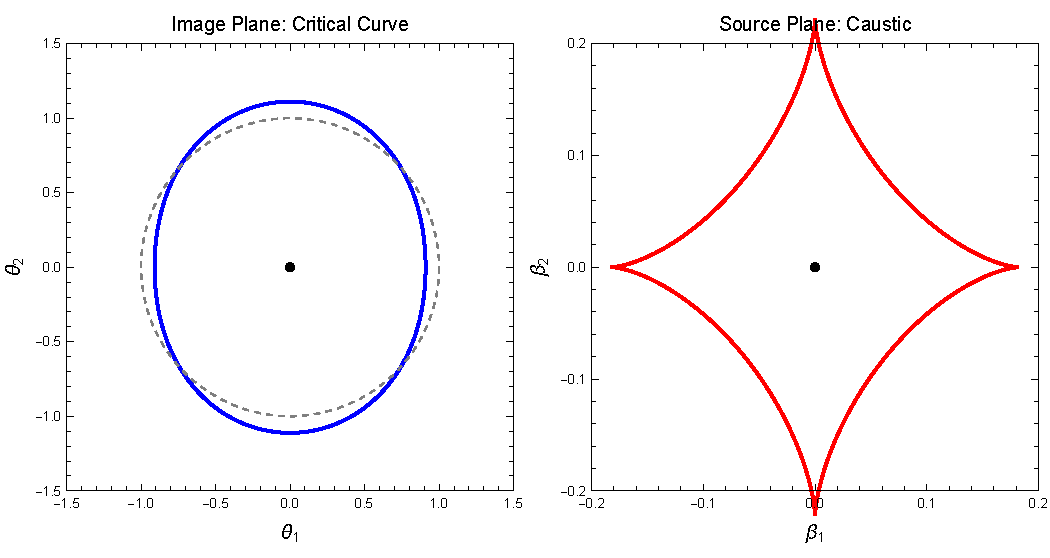
\includegraphics[width=0.85\textwidth]{../Figures/08_Elliptical_Models_Caustics/sis_shear_critical_caustic.pdf}
    \caption{Critical curves (left, image plane) and caustics (right,
    source plane) for the SIS + external shear model with
    $\thetaE = 1''$ and $\gamma_{\mathrm{ext}} = 0.1$.  The critical
    curve is an ellipse; the caustic is a diamond (astroid) with four
    cusps.  The shear axis is horizontal.
    Generated by \texttt{critical\_curves\_caustics.wl}.}
    \label{fig:sis_shear_crit_caust}
\end{figure}

\subsection{Image Configurations}

The image configurations for the SIS + shear model depend on the
source position relative to the diamond caustic:
\begin{itemize}
    \item \textbf{Source outside the diamond:} Two images (a double).
          One image is outside the critical curve (Type~I, positive
          parity); the other is inside (Type~II, negative parity,
          demagnified).
    \item \textbf{Source inside the diamond:} Four images (a quad).
          Two images outside the critical curve (positive parity);
          two inside (negative parity).
    \item \textbf{Source on a fold:} Three images, with two of them
          merging on the critical curve (highly magnified).
    \item \textbf{Source on a cusp:} Three images, with the merging
          triplet producing a characteristic cusp configuration.
\end{itemize}

\begin{remark}
The SIS is singular, so there is no separate radial critical curve
or radial caustic.  The SIS + shear model therefore has only a
tangential caustic (the diamond).  A non-singular model (e.g., a
softened isothermal sphere + shear) would also have a radial caustic
enclosing the tangential one.
\end{remark}


% =====================================================================
\section{The Singular Isothermal Ellipsoid (SIE)}
\label{sec:sie}

The \textbf{singular isothermal ellipsoid} (SIE) is the workhorse
model for galaxy-scale strong lensing.  Rather than adding shear
externally, the SIE builds ellipticity directly into the mass
distribution.

\subsection{Surface Mass Density}

The SIE surface mass density is
(Kormann, Schneider \& Bartelmann 1994; Congdon \& Keeton eq.~6.15):
\begin{equation}
    \boxed{
    \Sigma(\xi_1, \xi_2)
    = \frac{\sigma_v^2}{2\Gnewton}
    \,\frac{\sqrt{q}}{\sqrt{\xi_1^2 + q^2\,\xi_2^2}}
    }
    \label{eq:sie_sigma}
\end{equation}
where $q \leq 1$ is the axis ratio ($q = b/a$, with $a$ the
semi-major axis aligned along $\xi_1$), $\sigma_v$ is the velocity
dispersion, and $(\xi_1, \xi_2)$ are physical coordinates in the
lens plane.  For $q = 1$ this reduces to the SIS surface mass
density $\Sigma = \sigma_v^2/(2\Gnewton\xi)$.

The iso-density contours are ellipses with axis ratio $q$.  The
factor $\sqrt{q}$ ensures that the total mass enclosed within a
given elliptical radius is consistent with the isothermal profile.

\subsection{Deflection Angle}

The deflection angle for the SIE was derived by Kormann et al.\ (1994)
and involves inverse trigonometric/hyperbolic functions:
\begin{equation}
    \boxed{
    \alpha_1 = \frac{\thetaE\,\sqrt{q}}{\sqrt{1 - q^2}}
    \,\mathrm{arctan}\!\left(
    \frac{\theta_1\,\sqrt{1 - q^2}}
    {\sqrt{q^2\theta_1^2 + \theta_2^2}}\right)
    }
    \label{eq:sie_alpha1}
\end{equation}
\begin{equation}
    \boxed{
    \alpha_2 = \frac{\thetaE\,\sqrt{q}}{\sqrt{1 - q^2}}
    \,\mathrm{arctanh}\!\left(
    \frac{\theta_2\,\sqrt{1 - q^2}}
    {\sqrt{q^2\theta_1^2 + \theta_2^2}}\right)
    }
    \label{eq:sie_alpha2}
\end{equation}
where $\thetaE = 4\pi\sigma_v^2\Dds/(\speedoflight^2\Ds)$ is the
Einstein radius of the corresponding SIS\@.  Note the asymmetry:
$\alpha_1$ involves $\mathrm{arctan}$ while $\alpha_2$ involves
$\mathrm{arctanh}$.  This asymmetry reflects the elliptical geometry.

\begin{remark}
For $q \to 1$ (circular limit), both deflection components reduce to
$\alpha_i \to \thetaE\,\theta_i/|\vectheta|$, recovering the SIS
result.  This can be verified by taking the limit
$\sqrt{1-q^2} \to 0$ and using $\mathrm{arctan}(x)/x \to 1$ and
$\mathrm{arctanh}(x)/x \to 1$ as $x \to 0$.
\end{remark}

\subsection{Critical Curves and Caustics of the SIE}

The critical curves of the SIE are found by solving
$\det\Amat(\vectheta) = 0$.  Unlike the SIS (where the critical
curve is a circle), the SIE critical curves are smooth oval curves
whose shape depends on $q$.

For axis ratios $q \lesssim 0.9$, the SIE has:
\begin{itemize}
    \item A \textbf{tangential critical curve}: a smooth oval close
          to the Einstein radius, elongated perpendicular to the
          mass distribution's major axis.
    \item A \textbf{tangential caustic}: a diamond (astroid) shape,
          similar to the SIS + shear case, with four cusps.
\end{itemize}

The SIE, being singular at the origin, does not have a radial
critical curve (just as the SIS does not).  A non-singular
isothermal ellipsoid would also have a radial critical curve mapping
to a radial caustic.

The cross-section for quad lensing (the area enclosed by the
tangential caustic) increases with ellipticity.  For $q = 0.7$, the
caustic area is roughly $0.04\,\thetaE^2$, while for $q = 0.5$ it
can be several times larger.  This is why more elliptical galaxies
are more likely to produce quad lens systems.

\begin{figure}[ht]
    \centering
    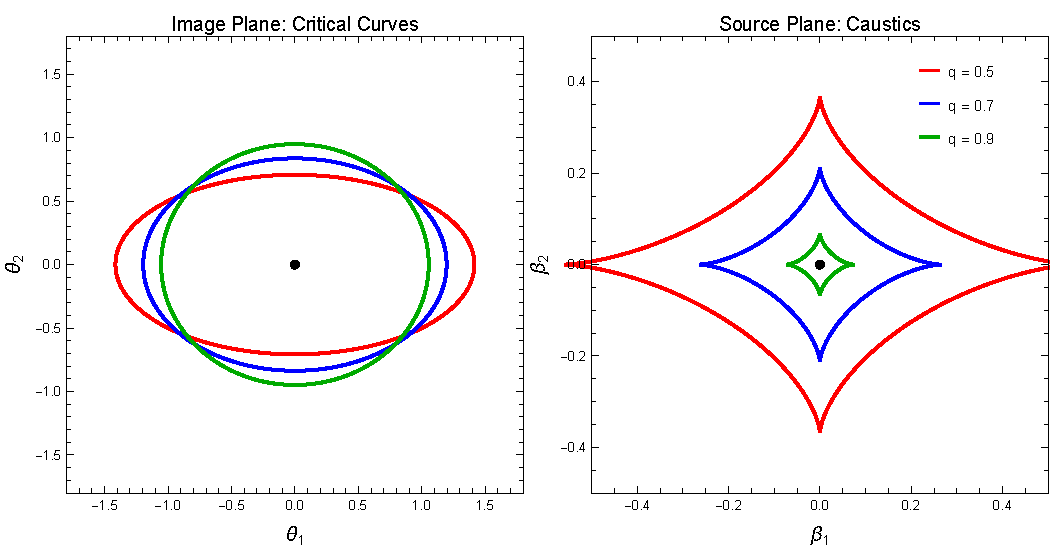
\includegraphics[width=0.85\textwidth]{../Figures/08_Elliptical_Models_Caustics/sie_critical_caustic.pdf}
    \caption{Critical curves (left) and caustics (right) for the SIE
    model with $\thetaE = 1''$ and axis ratios $q = 0.5$, $0.7$,
    and $0.9$.  As $q$ decreases (more elliptical), the diamond
    caustic grows larger, increasing the cross-section for
    quad imaging.
    Generated by \texttt{critical\_curves\_caustics.wl}.}
    \label{fig:sie_crit_caust}
\end{figure}


% =====================================================================
\section{Critical Curves}
\label{sec:critical_curves}

We now develop the general theory of critical curves, building on
the preview in Module~\ref{ch:magnification}
(Section~\ref{sec:critical_curves_preview}).

\begin{definition}
The \textbf{critical curves} are the loci in the image plane where
the Jacobian determinant vanishes:
\begin{equation}
    \boxed{
    \det\Amat(\vectheta) = 0
    \qquad \Longleftrightarrow \qquad
    (1 - \kappab)^2 - |\gammaL|^2 = 0
    }
    \label{eq:critical_curve_def}
\end{equation}
Equivalently, $\mu(\vectheta) \to \infty$ on critical curves.
\end{definition}

\subsection{Two Families of Critical Curves}

Using the eigenvalues $\lambda_\pm = 1 - \kappab \pm |\gammaL|$ of
the Jacobian (Module~\ref{ch:magnification}, eq.~\ref{eq:eigenvalues}),
the condition $\det\Amat = \lambda_+\,\lambda_- = 0$ is satisfied
when either eigenvalue vanishes:

\begin{enumerate}
    \item \textbf{Tangential critical curve} ($\lambda_- = 0$):
    \begin{equation}
        1 - \kappab(\vectheta) = |\gammaL(\vectheta)|
        \label{eq:tangential_crit}
    \end{equation}
    Images near this curve are stretched \textit{tangentially}
    (along the curve), because the eigenvalue corresponding to the
    tangential direction vanishes.  Giant arcs in clusters trace the
    tangential critical curve.

    \item \textbf{Radial critical curve} ($\lambda_+ = 0$):
    \begin{equation}
        1 - \kappab(\vectheta) = -|\gammaL(\vectheta)|
        \label{eq:radial_crit}
    \end{equation}
    Images near this curve are stretched \textit{radially}
    (perpendicular to the curve).  Radial arcs (pointing toward the
    lens center) form near radial critical curves, though they are
    rarer and fainter than tangential arcs.
\end{enumerate}

\subsection{Critical Curves for Axisymmetric vs.\ Elliptical Lenses}

\begin{itemize}
    \item \textbf{Axisymmetric lenses:} The critical curves are
          circles centered on the lens.  For the SIS, there is only
          a tangential critical curve at $\theta = \thetaE$.  For
          the point mass, the critical curve is the Einstein ring.
    \item \textbf{Elliptical lenses:} The critical curves become
          ellipses or ovals.  The tangential critical curve is
          typically elongated perpendicular to the lens ellipticity
          axis.  The shapes are computed numerically by solving
          $\det\Amat = 0$ on a grid or parametrically.
\end{itemize}

\subsection{Physical Meaning}

Critical curves are the sites of maximum magnification.  Images that
form near a critical curve are:
\begin{enumerate}
    \item \textbf{Highly magnified:} $|\mu| \gg 1$, because
          $\det\Amat \approx 0$.
    \item \textbf{Highly stretched:} Along one direction (tangential
          or radial), the magnification diverges while it remains
          finite in the orthogonal direction.  This produces the
          elongated arc morphology.
    \item \textbf{On parity boundaries:} As we cross a critical
          curve, $\det\Amat$ changes sign, so the image parity
          flips.  One side has positive parity (Type~I); the other
          has negative parity (Type~II).
\end{enumerate}

The practical significance is enormous: critical curves are where we
look for the most highly magnified background sources.  Cluster
lensing surveys map out critical curves to find magnified galaxies at
very high redshift.


% =====================================================================
\section{Caustics}
\label{sec:caustics}

\begin{definition}
The \textbf{caustics} are the images of the critical curves under the
lens mapping.  That is, the caustics are the curves in the
\textit{source plane} obtained by applying the lens equation to each
point on a critical curve:
\begin{equation}
    \boxed{
    \vecbeta_{\mathrm{caustic}}
    = \vectheta_{\mathrm{crit}}
    - \vecalpha(\vectheta_{\mathrm{crit}})
    }
    \label{eq:caustic_def_mod8}
\end{equation}
\end{definition}

\subsection{Types of Caustics}

Corresponding to the two families of critical curves, there are two
types of caustics:

\begin{enumerate}
    \item \textbf{Tangential caustic:} The mapping of the tangential
          critical curve.  For elliptical lenses, this is typically a
          diamond (astroid) shape with four cusps.  Sources inside
          the tangential caustic are quadruply imaged.

    \item \textbf{Radial caustic:} The mapping of the radial
          critical curve.  This is typically a smooth, roughly
          elliptical curve that encloses the tangential caustic.
          Sources inside the radial caustic but outside the
          tangential caustic are doubly imaged; sources outside both
          caustics have a single image.
\end{enumerate}

\subsection{Caustics for Specific Models}

\begin{itemize}
    \item \textbf{Point mass:} The tangential critical curve (Einstein
          ring $\theta = \thetaE$) maps to a single point
          ($\beta = 0$) --- a \textbf{degenerate point caustic}.  A
          source at $\beta = 0$ produces the Einstein ring; any
          source at $\beta > 0$ produces exactly two images.

    \item \textbf{SIS:} Same as the point mass --- the critical curve
          $\theta = \thetaE$ maps to $\beta = 0$.  The SIS has no
          radial caustic.  Sources with $\beta < \thetaE$ produce two
          images; sources with $\beta > \thetaE$ produce one image.

    \item \textbf{SIS + shear:} The tangential caustic opens up into
          a diamond (astroid) with four cusps.  The diamond size is
          proportional to $\gamma_{\mathrm{ext}}$.

    \item \textbf{SIE:} Same diamond structure as SIS + shear, with
          the diamond size controlled by the ellipticity $(1 - q)$.

    \item \textbf{Non-singular models} (NIS, NFW): Both tangential
          and radial caustics are present.  The radial caustic
          encloses the tangential one, creating regions with 1, 3,
          and 5 images.
\end{itemize}


% =====================================================================
\section{Image Topology}
\label{sec:image_topology}

This section is the conceptual heart of strong gravitational lensing.
It explains \textit{why} images appear and disappear as a source
moves, why they always come in pairs, and how the full image
configuration (positions, parities, magnifications) is determined
entirely by the source's location relative to the caustic structure.

The key insight is that \textbf{caustics are the boundaries between
regions of different image multiplicity}, and \textbf{critical curves
are the boundaries between regions of different image parity}.
Together, they provide a complete topological description of the
lens mapping.


\subsection{Critical Curves as Parity Boundaries}
\label{sec:parity_boundaries}

Recall from Module~\ref{ch:magnification} that the magnification is
$\mu = 1/\det\Amat$ and that the sign of $\mu$ determines the image
parity:
\begin{itemize}
    \item $\det\Amat > 0 \;\Rightarrow\; \mu > 0$: \textbf{positive
          parity} (Type~I image).  The image has the same orientation
          as the source.
    \item $\det\Amat < 0 \;\Rightarrow\; \mu < 0$: \textbf{negative
          parity} (Type~II image).  The image is mirror-reflected
          relative to the source.
\end{itemize}

Since $\det\Amat$ is a continuous function of position that passes
through zero on critical curves, the sign of $\det\Amat$ must
\textit{change} across a critical curve.  Therefore:

\begin{proposition}
\textbf{Critical curves are parity boundaries.}  Images on opposite
sides of a critical curve have opposite parities.  If a critical
curve separates region $R_+$ ($\det\Amat > 0$) from region $R_-$
($\det\Amat < 0$), then:
\begin{itemize}
    \item Images in $R_+$ have positive parity (Type~I, minima of the
          arrival time surface).
    \item Images in $R_-$ have negative parity (Type~II, saddle points
          of the arrival time surface).
\end{itemize}
\end{proposition}

For a typical galaxy lens with an elliptical mass distribution:
\begin{itemize}
    \item The region \textbf{outside} the tangential critical curve
          has $\det\Amat > 0$: images here are Type~I (positive
          parity, time-delay minima).
    \item The region \textbf{between} the tangential and radial
          critical curves has $\det\Amat < 0$: images here are
          Type~II (negative parity, saddle points).
    \item The region \textbf{inside} the radial critical curve has
          $\det\Amat > 0$ again: images here are Type~I or Type~III
          (positive parity, but corresponding to time-delay maxima
          for Type~III, as discussed in Module~\ref{ch:fermat_time_delays}).
\end{itemize}

\begin{remark}
The connection to Morse theory (Module~\ref{ch:fermat_time_delays})
is direct.  The three image types correspond to the three types of
stationary points of the Fermat potential: \textbf{Type~I} = minimum,
\textbf{Type~II} = saddle, \textbf{Type~III} = maximum.  The
magnification parity determines the Morse index.
\end{remark}


\subsection{Caustic Crossings and Image Creation/Destruction}
\label{sec:caustic_crossings}

The most important property of caustics is:

\begin{proposition}
\textbf{Image creation/destruction at caustics.}  When a source
crosses a caustic, the number of images changes by exactly two.  A
pair of images either \textbf{appears} (as the source enters a
higher-multiplicity region) or \textbf{disappears} (as it exits).
\end{proposition}

This happens because, as a source approaches a caustic from the side
with fewer images, two of the ``potential'' image positions on
opposite sides of the corresponding critical curve converge toward
the critical curve.  At the moment the source is exactly on the
caustic, the two images merge \textit{on} the critical curve (where
$\det\Amat = 0$ and the magnification diverges).  As the source
crosses the caustic, the two images separate and become distinct.

Crucially, the two images that appear or disappear:
\begin{enumerate}
    \item Are located on \textbf{opposite sides} of the critical
          curve.
    \item Have \textbf{opposite parities} (one Type~I, one Type~II).
    \item Are both \textbf{highly magnified} near the caustic
          (their magnifications diverge as they approach the critical
          curve).
    \item Have \textbf{nearly equal magnifications} (in absolute
          value) near the caustic.
\end{enumerate}

\begin{remark}
The fact that images always appear or disappear in \textbf{pairs}
with opposite parities is a topological necessity.  It preserves
\textbf{Burke's odd-number theorem}
(Module~\ref{ch:fermat_time_delays}): the total number of images is
always odd (for a non-singular, transparent lens with a source
inside the outermost caustic).  Since images are created and
destroyed in pairs, the parity of the count (odd or even) never
changes.
\end{remark}


\subsection{Walking a Source Across Caustics: A Worked Example}
\label{sec:source_walk}

To make the image creation/destruction process concrete, we walk
through a complete example using an SIE lens with axis ratio
$q = 0.7$ and Einstein radius $\thetaE = 1''$.  The SIE has a
tangential caustic (diamond shape) in the source plane.  For a
non-singular model there would also be a radial caustic enclosing
the diamond, but for the SIE (which is singular at the center) we
focus on the tangential caustic.

Consider a source that starts far from the lens and moves inward,
crossing the caustics:

\paragraph{Stage 1: Source far outside all caustics.}
The source position $\vecbeta$ is far from the lens center, well
outside any caustic.  There is \textbf{one image} (for singular
models like the SIE, there are actually two images even here, but
the second is extremely demagnified near the lens center and is
often unobservable).  The observable image is:
\begin{itemize}
    \item \textbf{Type~I} (positive parity, minimum of the arrival
          time).
    \item Located outside the tangential critical curve, near the
          true source position.
    \item Weakly magnified ($|\mu| \approx 1$).
\end{itemize}

\paragraph{Stage 2: Source crosses the tangential caustic (outside
$\to$ inside).}
As the source reaches the tangential (diamond) caustic, two new
images appear simultaneously, straddling the tangential critical
curve.  The total count goes from \textbf{1 to 3 images}
(or effectively from 2 to 4, counting the faint central image):
\begin{enumerate}
    \item The \textbf{original Type~I image} (positive parity,
          outside the tangential critical curve) persists, moving
          slightly.
    \item A \textbf{new Type~II image} (negative parity) appears
          just inside the tangential critical curve.  This is a
          \textit{saddle point} of the arrival time surface.  It is
          highly magnified and tangentially stretched.
    \item A \textbf{new Type~I image} (positive parity) appears
          just outside the tangential critical curve, close to the
          Type~II image.  This is a \textit{minimum} of the
          arrival time surface.  It is also highly magnified.
\end{enumerate}

The two new images are born as a highly magnified, closely spaced
pair straddling the critical curve.  They have opposite parities
(one positive, one negative) and nearly equal $|\mu|$.  As the
source moves further inside the caustic, they separate and their
magnifications decrease.

\paragraph{Stage 3: Source inside the tangential caustic (quad
configuration).}
With the source well inside the diamond caustic, four bright images
surround the lens (plus a faint, highly demagnified central image in
non-singular models).  The typical configuration is an
\textbf{Einstein cross}:
\begin{itemize}
    \item Two Type~I images (positive parity, outside the tangential
          critical curve).
    \item Two Type~II images (negative parity, inside the tangential
          critical curve).
\end{itemize}

The four images form a roughly cross-shaped pattern around the lens.
The magnification depends on the source's proximity to the caustic
folds and cusps.

\paragraph{Stage 4: Source crosses the tangential caustic again
(inside $\to$ outside).}
As the source exits the diamond caustic, two images converge on the
critical curve, merge, and disappear.  The count drops from
\textbf{3 back to 1} (or 4 to 2 counting the central image).  The
two images that disappear are a Type~I/Type~II pair, just as in the
creation event.

\begin{figure}[ht]
    \centering
    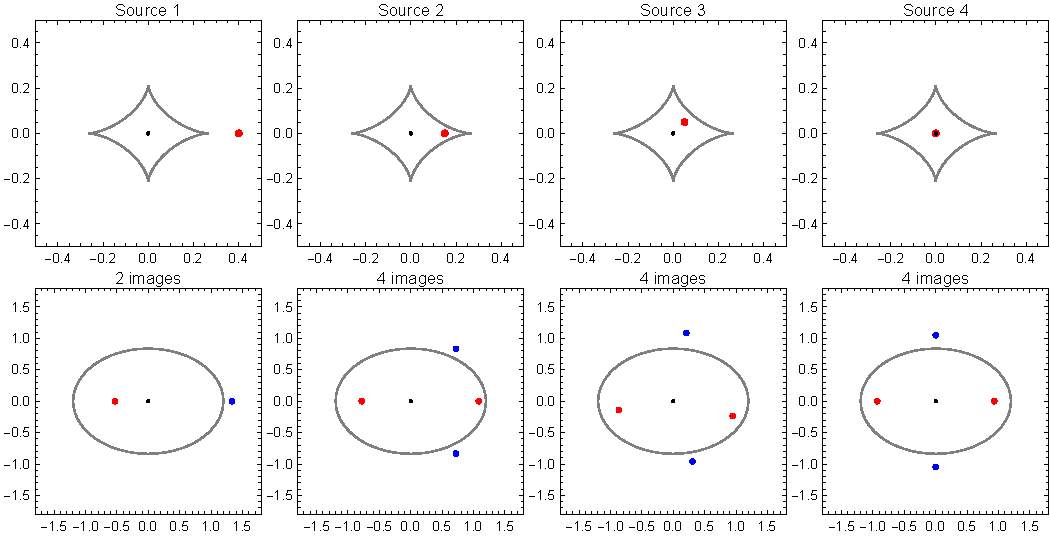
\includegraphics[width=0.95\textwidth]{../Figures/08_Elliptical_Models_Caustics/source_walk_caustic.pdf}
    \caption{A source walks across the caustic of an SIE lens
    ($q = 0.7$).  \textbf{Top row:} Source positions (red star) in
    the source plane, with the diamond caustic shown.
    \textbf{Bottom row:} Corresponding image configurations in the
    image plane, with the critical curve shown.  Blue circles =
    Type~I images (positive parity); red squares = Type~II images
    (negative parity).  As the source crosses the caustic, images
    appear/disappear in pairs.
    Generated by \texttt{critical\_curves\_caustics.wl}.}
    \label{fig:source_walk}
\end{figure}

For a non-singular lens model (e.g., a softened isothermal
ellipsoid), there is also a \textbf{radial caustic} enclosing the
tangential one.  As the source crosses the radial caustic inward,
two additional images appear near the radial critical curve (near
the lens center), bringing the total from 3 to 5.  This gives the
complete sequence:
\begin{center}
\begin{tabular}{ccccc}
\toprule
\textbf{Region} & \textbf{Image count} & \textbf{Types} \\
\midrule
Outside radial caustic & 1 & I \\
Between radial \& tangential & 3 & I, II, III \\
Inside tangential caustic & 5 & I, I, II, II, III \\
\bottomrule
\end{tabular}
\end{center}
Here Type~III is a maximum of the arrival time (the highly
demagnified central image).


\subsection{The Fold and Cusp Catastrophes}
\label{sec:fold_cusp}

The caustic curves of a generic smooth lens consist of two types of
points: \textbf{folds} (smooth segments) and \textbf{cusps} (pointed
corners).  These are the only two generic singularities of smooth
two-dimensional mappings, a result from \textbf{catastrophe theory}
(or singularity theory; see Petters, Levine \& Wambsganss 2001 for
a thorough treatment).

\subsubsection{Fold Caustics}

Near a \textbf{fold} (a smooth segment of the caustic), the
following properties hold:

\begin{enumerate}
    \item \textbf{Two images merge.}  As a source crosses a fold
          caustic, two images appear or disappear.  The images
          straddle the critical curve, one on each side.

    \item \textbf{Magnification scaling.}  Near a fold, the
          magnification of each of the two merging images scales as:
    \begin{equation}
        \boxed{
        |\mu| \propto \frac{1}{\sqrt{d_{\perp}}}
        }
        \label{eq:fold_magnification}
    \end{equation}
    where $d_\perp$ is the perpendicular distance of the source
    from the caustic.  The magnification diverges as
    $d_\perp \to 0$ (source on the caustic), but only as an
    inverse square root --- a relatively mild divergence.

    \item \textbf{Equal and opposite magnifications.}  The two
          merging images have magnifications that approach
          $+|\mu_0|$ and $-|\mu_0|$ (equal absolute values,
          opposite signs), so their \textit{total signed
          magnification} approaches zero.  The unsigned total
          $2|\mu_0| \propto 1/\sqrt{d_\perp}$ diverges.

    \item \textbf{Tangential stretching.}  The merging images are
          highly elongated tangentially (along the critical curve)
          and compressed radially.  This is the origin of the
          ``arc'' morphology.
\end{enumerate}

\subsubsection{Cusp Caustics}

Near a \textbf{cusp} (a pointed corner of the caustic), the behavior
is richer:

\begin{enumerate}
    \item \textbf{Three images merge.}  As a source approaches a
          cusp from inside the caustic, three images converge toward
          a single point on the critical curve.  These form the
          characteristic \textbf{cusp triplet}.

    \item \textbf{Stronger magnification divergence.}  Near a cusp,
          the total magnification diverges more strongly than for a
          fold.  The scaling is:
    \begin{equation}
        \mu_{\mathrm{total}} \propto d_{\perp}^{-1}
        \label{eq:cusp_magnification}
    \end{equation}
    (compared to $d_\perp^{-1/2}$ for a fold).

    \item \textbf{Cusp relation.}  The magnifications of the three
          cusp images satisfy a relation:
    \begin{equation}
        \mu_A + \mu_B + \mu_C \approx 0
        \label{eq:cusp_relation}
    \end{equation}
    where $A$, $B$, $C$ are the three images of the cusp triplet
    (with signed magnifications).  That is, the sum of the signed
    magnifications of the three brightest images in a cusp
    configuration should vanish.  Violations of this relation
    indicate substructure (e.g., dark matter subhalos) perturbing
    the images.

    \item \textbf{Configuration.}  The three cusp images are
          closely spaced along the critical curve.  One is on the
          opposite side of the critical curve from the other two,
          ensuring opposite parities.
\end{enumerate}

\begin{remark}
The fold and cusp are the only \textbf{stable} (generic)
singularities of smooth two-dimensional maps.  Higher-order
singularities (swallowtails, lips, etc.)\ require special symmetries
or fine-tuning and are not generically present in gravitational lens
models.  This is a deep result of Whitney's theorem in singularity
theory (Petters et al.\ 2001, Ch.~5--6).
\end{remark}

\begin{figure}[ht]
    \centering
    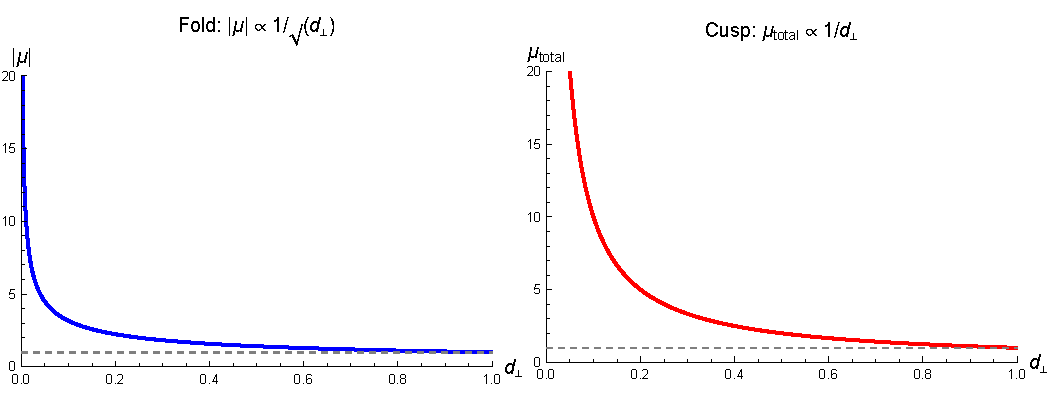
\includegraphics[width=0.85\textwidth]{../Figures/08_Elliptical_Models_Caustics/fold_cusp_magnification.pdf}
    \caption{Magnification behavior near fold and cusp caustics.
    \textbf{Left:} Near a fold, two images straddle the critical
    curve with magnifications scaling as $|\mu| \propto
    1/\sqrt{d_\perp}$.
    \textbf{Right:} Near a cusp, three images merge, with stronger
    divergence.  The cusp relation $\mu_A + \mu_B + \mu_C \approx 0$
    holds for the signed magnifications.
    Generated by \texttt{critical\_curves\_caustics.wl}.}
    \label{fig:fold_cusp}
\end{figure}


\subsection{Image Configuration Taxonomy}
\label{sec:image_taxonomy}

The caustic structure of a lens determines all possible image
configurations.  For an elliptical galaxy lens (SIE or similar model),
the following taxonomy applies:

\subsubsection{Doubles}

\textbf{Source outside the tangential caustic.}  Two images form (or
effectively one bright image plus one highly demagnified image near
the lens center for singular models):
\begin{itemize}
    \item One Type~I image (positive parity, outside the critical
          curve): the dominant, brighter image.
    \item One Type~II image (negative parity, inside the critical
          curve): typically fainter, on the opposite side of the
          lens from the source.
\end{itemize}
Doubles account for $\sim$70--80\% of known galaxy-scale lens
systems.

\subsubsection{Quads / Einstein Crosses}

\textbf{Source inside the tangential caustic.}  Four bright images
form (plus a faint central image):
\begin{itemize}
    \item Two Type~I images (positive parity), roughly on the side
          of the lens closer to the source.
    \item Two Type~II images (negative parity), on the opposite
          side.
\end{itemize}
The four images form a roughly cross-shaped (\textbf{Einstein cross})
or diamond-shaped pattern around the lens.  Quads account for
$\sim$20--30\% of galaxy-scale systems and are extremely valuable
for cosmography because they provide three independent time delays.

\subsubsection{Cusp Configurations}

\textbf{Source near a cusp of the tangential caustic.}  Three of the
four images in a quad merge into a closely spaced triplet near one
point on the critical curve.  This produces the \textbf{naked cusp}
or \textbf{cusp triplet} configuration:
\begin{itemize}
    \item Three closely spaced images near the cusp of the critical
          curve, with the cusp relation
          $\mu_A + \mu_B + \mu_C \approx 0$.
    \item One isolated image on the opposite side of the lens.
\end{itemize}

\subsubsection{Why Most Observed Quads Have a Diamond Caustic}

The tangential caustic of an elliptical galaxy lens is generically a
diamond (astroid) shape.  This is because:
\begin{enumerate}
    \item The dominant perturbation from circular symmetry is
          quadrupolar (ellipticity or shear), which produces
          exactly four cusps.
    \item Higher-order multipoles (hexapole, octupole) are typically
          subdominant and do not change the topology of the caustic.
    \item The diamond caustic produces Einstein crosses (quads with
          roughly equal magnifications) when the source is near the
          center, and fold/cusp configurations when the source is
          near a fold or cusp of the diamond.
\end{enumerate}


\subsection{Why Giant Arcs Form}
\label{sec:giant_arcs_preview}

One of the most spectacular phenomena in strong lensing is the
formation of \textbf{giant luminous arcs} in galaxy clusters.  The
theory of critical curves and caustics provides a complete
explanation.

\paragraph{Step 1: Sources near the tangential caustic.}
Giant arcs form when a background galaxy lies very close to (but
just inside or outside) the tangential caustic.  At this location,
one or two of its images lie very close to the tangential critical
curve.

\paragraph{Step 2: Tangential stretching near the critical curve.}
The tangential critical curve is where $\lambda_- = 0$ (the
eigenvalue corresponding to the tangential direction vanishes).
Near this curve, images are stretched enormously in the
\textit{tangential} direction (along the critical curve) while
remaining relatively unstretched in the radial direction.

Quantitatively, if the source is at perpendicular distance
$d_\perp$ from the tangential caustic, the tangential magnification
scales as:
\begin{equation}
    \mu_{\mathrm{tan}} \propto \frac{1}{\sqrt{d_\perp}}
    \label{eq:tangential_magnification}
\end{equation}
while the radial magnification remains of order unity.  The result
is an image that is stretched by a factor of $\mu_{\mathrm{tan}}$
along the critical curve but not radially --- an \textbf{arc}.

\paragraph{Step 3: Arc length and curvature.}
Since the arc follows the tangential critical curve, its curvature
matches that of the critical curve.  For a galaxy cluster, the
tangential critical curve has a radius of $\sim$10--30 arcsec, so
giant arcs appear as curved features with large opening angles.
The length-to-width ratio of the arc is approximately
$\mu_{\mathrm{tan}} \sim 1/\sqrt{d_\perp}$, which can easily reach
10:1 or more for sources very close to the caustic.

\paragraph{Step 4: Multiple arcs.}
A source just inside the tangential caustic produces two highly
magnified images on opposite sides of the tangential critical curve
(a fold pair).  Both images are arcs.  If the source is also near a
cusp, three images merge into a very long arc (a ``cusp arc'').

\begin{remark}
The largest known arcs in galaxy clusters have length-to-width ratios
exceeding 10:1 and total magnifications of $\mu \sim 20$--50.  These
extreme magnifications are used to study intrinsically faint galaxies
at high redshift (``cosmic telescopes'').
\end{remark}


% =====================================================================
\section{Image Configurations: Doubles, Quads, and Einstein Crosses}
\label{sec:image_configurations}

We now illustrate the different image configurations with explicit
examples for an SIE lens.

\subsection{Double Configuration}

For a source at $\vecbeta = (0.5, 0.0)''$ lensed by an SIE with
$\thetaE = 1''$, $q = 0.7$:  The source is outside the tangential
caustic.  Two images form:
\begin{itemize}
    \item Image A at $\vectheta_A \approx (1.35, 0.0)''$: Type~I,
          positive parity, $\mu_A \approx 2.5$.
    \item Image B at $\vectheta_B \approx (-0.65, 0.0)''$: Type~II,
          negative parity, $\mu_B \approx -0.9$.
\end{itemize}
The brighter image (A) is on the same side as the source; the
fainter image (B) is on the opposite side.

\subsection{Quad / Einstein Cross Configuration}

For a source at $\vecbeta = (0.05, 0.05)''$ (inside the tangential
caustic):  Four bright images form, arranged in a cross pattern.
The two Type~I images tend to be on the side closer to the source;
the two Type~II images are on the opposite side.  The magnifications
of the four images are comparable, with the images nearer the
critical curve being brighter.

\subsection{Cusp Configuration}

For a source near a cusp of the tangential caustic (e.g., near
$\vecbeta \approx (0.15, 0.0)''$ for an SIE with $q = 0.7$):
Three images cluster together near the corresponding point on the
critical curve, forming a cusp triplet.  The fourth image is
isolated on the opposite side.

\begin{figure}[ht]
    \centering
    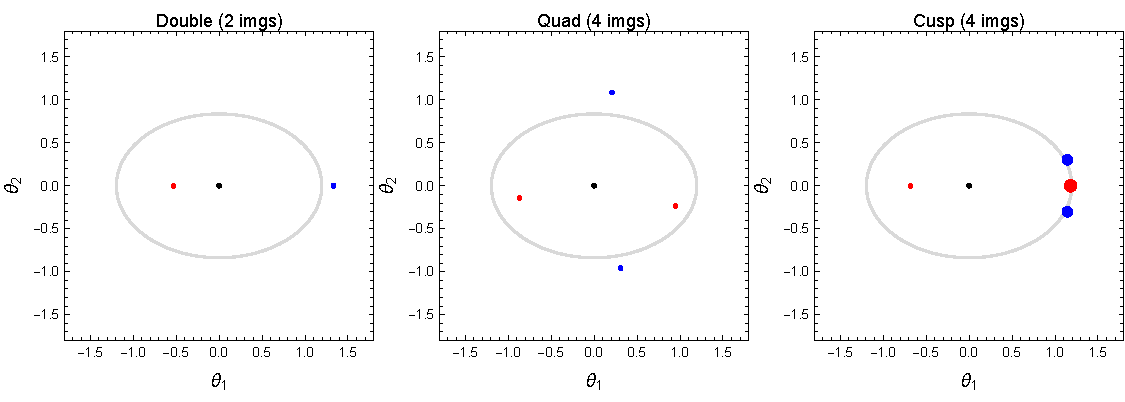
\includegraphics[width=0.95\textwidth]{../Figures/08_Elliptical_Models_Caustics/image_configurations.pdf}
    \caption{Image configurations for an SIE lens with
    $\thetaE = 1''$ and $q = 0.7$.  \textbf{Left:} Double (source
    outside caustic).  \textbf{Center:} Quad / Einstein cross
    (source inside caustic).  \textbf{Right:} Cusp configuration
    (source near a cusp).  Blue = Type~I (positive parity);
    red = Type~II (negative parity).  The critical curve and
    caustic are shown as gray curves.
    Generated by \texttt{critical\_curves\_caustics.wl}.}
    \label{fig:image_configs}
\end{figure}


% =====================================================================
\section{Summary}
\label{sec:elliptical_summary}

\begin{itemize}
    \item \textbf{SIS + external shear} is the simplest
          non-axisymmetric model.  The external shear
          $\gamma_{\mathrm{ext}}$ deforms the critical curve into an
          ellipse and opens the point caustic into a
          \textbf{diamond (astroid)} with four cusps.

    \item The \textbf{singular isothermal ellipsoid} (SIE) builds
          ellipticity directly into the mass distribution.  Its
          deflection angle involves $\arctan$ and $\mathrm{arctanh}$
          functions (Kormann et al.\ 1994).  It is the standard model
          for galaxy-scale lens modeling.

    \item \textbf{Critical curves} ($\det\Amat = 0$) are parity
          boundaries in the image plane.  The tangential critical
          curve ($1 - \kappab = |\gammaL|$) is the site of giant arcs;
          the radial critical curve ($1 - \kappab = -|\gammaL|$) is
          the site of radial arcs.

    \item \textbf{Caustics} are the mappings of critical curves to
          the source plane.  They divide the source plane into regions
          of different image multiplicity.

    \item \textbf{Image topology:}  As a source crosses a caustic,
          two images appear or disappear on opposite sides of the
          critical curve, with opposite parities.  This preserves
          Burke's odd-number theorem.

    \item \textbf{Fold caustics:}  Two images merge; magnification
          $|\mu| \propto 1/\sqrt{d_\perp}$.  This produces giant
          arcs.

    \item \textbf{Cusp caustics:}  Three images merge; the cusp
          relation $\mu_A + \mu_B + \mu_C \approx 0$ holds.

    \item \textbf{Image configurations:}  Doubles (source outside
          caustic), quads/Einstein crosses (source inside caustic),
          and cusp triplets (source near a cusp) account for the
          observed morphologies of strong lens systems.

    \item \textbf{Giant arcs} form when extended sources lie near the
          tangential caustic: images are tangentially stretched by
          factors of $\mu_{\mathrm{tan}} \propto 1/\sqrt{d_\perp}$
          along the tangential critical curve.
\end{itemize}


% =====================================================================
\section{Problems}
\label{sec:elliptical_problems}

\begin{exercise}
\label{ex:sis_shear_crit}
\textbf{(SIS + shear: critical curves and caustics.)}
Consider an SIS + external shear model with $\thetaE = 1''$ and
$\gamma_{\mathrm{ext}} = 0.1$.
\begin{enumerate}[label=(\alph*)]
    \item Starting from the lensing potential
          (eq.~\ref{eq:psi_sis_shear}), compute the Jacobian matrix
          $\Amat$ and the determinant $\det\Amat$ as functions of
          $(\theta_1, \theta_2)$.
    \item Solve $\det\Amat = 0$ to find the critical curve.  Express
          the result in polar coordinates $\theta_{\mathrm{crit}}(\phi)$.
          Plot the critical curve.
    \item Map the critical curve through the lens equation to obtain
          the caustic.  Plot the caustic in the source plane.  Verify
          that it has four cusps and the shape of an astroid.
    \item Estimate the area enclosed by the caustic (the quad
          cross-section).
\end{enumerate}
Verify with
\solnlink{08_Elliptical_Models_Caustics/problems\_08.wl}{problems\_08.wl}.
\end{exercise}

\begin{exercise}
\label{ex:sie_caustic}
\textbf{(SIE tangential caustic.)}
For an SIE with $\thetaE = 1''$ and axis ratio $q = 0.7$:
\begin{enumerate}[label=(\alph*)]
    \item Write down the deflection angle components $\alpha_1$ and
          $\alpha_2$ from eqs.~\eqref{eq:sie_alpha1}--\eqref{eq:sie_alpha2}.
    \item Compute the tangential caustic numerically by: (i)~finding
          the critical curve from $\det\Amat = 0$, and (ii)~mapping
          it through the lens equation.  Plot the caustic.
    \item Compute the area of the tangential caustic (the quad
          cross-section) numerically.  How does it compare to the
          SIS + shear model with the same effective ellipticity?
\end{enumerate}
Verify with
\solnlink{08_Elliptical_Models_Caustics/problems\_08.wl}{problems\_08.wl}.
\end{exercise}

\begin{exercise}
\label{ex:fold_magnification}
\textbf{(Fold magnification scaling.)}
Show that images appear or disappear in pairs at caustic crossings
by analyzing $\det\Amat$ near a fold:
\begin{enumerate}[label=(\alph*)]
    \item Near a fold caustic, the lens mapping in the direction
          perpendicular to the fold can be approximated as
          $\beta_\perp \approx a\,\theta_\perp^2$, where
          $\theta_\perp$ is the signed distance from the critical
          curve and $a$ is a constant.  Show that for
          $\beta_\perp > 0$, there are two solutions
          $\theta_\perp = \pm\sqrt{\beta_\perp/a}$ (one on each
          side of the critical curve), while for $\beta_\perp < 0$
          there are no solutions.
    \item Compute the Jacobian of the simplified mapping and show
          that the magnification scales as
          $|\mu| \propto 1/\sqrt{\beta_\perp}$ for each image.
    \item Show that the two images have opposite parities
          (opposite signs of $\det\Amat$).
\end{enumerate}
Verify with
\solnlink{08_Elliptical_Models_Caustics/problems\_08.wl}{problems\_08.wl}.
\end{exercise}

\begin{exercise}
\label{ex:sie_images}
\textbf{(SIE image positions.)}
For a source at $\vecbeta = (0.1, 0.2)''$ lensed by an SIE with
$\thetaE = 1''$ and $q = 0.8$:
\begin{enumerate}[label=(\alph*)]
    \item Determine whether the source is inside or outside the
          tangential caustic.  How many images do you expect?
    \item Find all image positions $\vectheta_i$ numerically by
          solving the lens equation
          $\vecbeta = \vectheta - \vecalpha(\vectheta)$.
    \item For each image, compute the magnification $\mu_i$ and
          determine the parity (Type~I or Type~II).
    \item Compute the signed magnification sum $\sum_i \mu_i$ and
          discuss whether it is consistent with the expected value
          (considering the missing central image for the singular SIE).
\end{enumerate}
Verify with
\solnlink{08_Elliptical_Models_Caustics/problems\_08.wl}{problems\_08.wl}.
\end{exercise}

\begin{exercise}
\label{ex:burke_verification}
\textbf{(Burke's odd-number theorem for the SIE.)}
Verify Burke's odd-number theorem for an SIE with $\thetaE = 1''$
and $q = 0.7$:
\begin{enumerate}[label=(\alph*)]
    \item For a source outside the tangential caustic (e.g.,
          $\vecbeta = (0.5, 0.0)''$), find all image positions.
          Count the images (including any faint central image) and
          verify the count is odd.
    \item For a source inside the tangential caustic (e.g.,
          $\vecbeta = (0.05, 0.05)''$), find all image positions.
          Verify the count is odd.
    \item For each case, classify each image by parity and verify
          that the number of positive-parity images exceeds the
          number of negative-parity images by one.
    \item Discuss why the SIE (being singular at the origin)
          requires care in applying Burke's theorem.  What role does
          the central image play?
\end{enumerate}
Verify with
\solnlink{08_Elliptical_Models_Caustics/problems\_08.wl}{problems\_08.wl}.
\end{exercise}
